\documentclass[a4paper, 11pt]{article}
\usepackage{graphicx}
\usepackage{fancyvrb}
\usepackage{algpseudocode}
\usepackage{float}
\usepackage{caption}
\usepackage{subcaption}
\usepackage [english]{babel}

\floatstyle{ruled}
\newfloat{file}{thp}{lop}
\floatname{file}{File}
\newfloat{algorithm}{thp}{lop}
\floatname{algorithm}{Algorithm}
 
\begin{document}
\title{Broadcast Simulator}
\author{Bruno Jurkovski \and Oscar Chavez}
\maketitle
 
\tableofcontents

\newpage 
\section{Introduction}

	Distributed systems are systems composed by several autonomous entities ($e.g.$ processes) each one with its own local memory. Since these entities want to do something useful together, they need a way to communicate and coordinate themselves. This is often done through the exchange of messages (using \texttt{send()} and \texttt{receive()} primitives).
	
	Besides exchanging simple messages with just one process, a process may also need to broadcast some information to all processes in a group. There are many different ways of that, depending on the assumptions about the environment (process crashes, network reliability, memory, etc) and on the properties that want to be ensured. For example, a few properties that are often designed by a broadcast protocol are:

\begin{description}
	\item[Agreement] if a correct process p delivers a message m, then all correct processes will deliver m.
	\item[Integrity] if a process delivers a message m, then m was sent by one process.
	\item[Validity] if a correct process sends a message, then it should eventually deliver it.
\end{description}

	Besides the assumptions and properties they ensure, protocols may also have differences regarding the performance metrics they try to optimize. Two common metrics used to evaluate the performance of these protocols are:

\begin{description}
	\item[Latency] the time it takes for a message to be delivered by all the process.
	\item[Throughput] the number of messages that can be delivered by instant of time.
\end{description}

	The choice of which broadcast protocol to use depends on the requirements of the application.

	The objective of this project is to:

\begin{enumerate}	
	\item Design and implement a single threaded, round based \textbf{simulator of broadcast protocols};
	\item Develop two \textbf{total order broadcast} protocols: one optimizing the latency and one optimizing the throughput.
\end{enumerate}
	
\newpage
\section{Simulator Implementation}
\subsection{Assumptions}
	A few assumptions were made during the implementation of the simulator (for all the protocols developed):

\begin{itemize}
	\item All the processes know each other;
	\item There are perfect point to point links: if a message \texttt{m} is sent by a correct process \texttt{p} to a correct process \texttt{q}, then \texttt{q} eventually delivers \texttt{m};
	\item There are no crashes;
	\item Ordinary messages are sent using \textit{unicast}, but acknowledgment messages can be sent using \textit{multicast};
	\item Ordinary messages and acknowledgments take the same time to be sent;
	\item Each process can deliver at most one message per round and send at most one message per round. If there are two messages that arrive to a process at the same round, they are queued in the process buffer and processed one at a time (round).
\end{itemize}

\subsection{Architecture}
	The system has two simulator classes: \textbf{BroadcastSimulator} and \textbf{TotalOrderBroadcastSimulator}. 
	
	The first one implements all the basic simulator behavior: controlling the processes and feeding them with new messages to be broadcasted (according to the configuration files explained in section \ref{subsec:usage}), and providing the processes with a network middleware (with the \texttt{send()} and \texttt{receive()} primitives)). 
	
	The second one extends the \texttt{send()} and \texttt{receive()} primitives to respond with acknowledgment messages and adds one logical clock per process (which makes it possible for the processes to embed a timestamp in each message and synchronize them).

	The simulators are implemented using a policy-based design. Both of the simulators described above receive a template parameter specifying the broadcast policy class to be used. The implemented classes are: \textbf{BasicPolicy}, \textbf{TreePolicy} and \textbf{PipelinePolicy}.
	
	Besides the simulator and the policy classes, there is one \textbf{Message} class (to model the messages exchanged by the processes) and one \textbf{SimulationLog} class (which stores all the messages sent and received at each round).


\subsection{Usage}
\label{subsec:usage}
	To execute the simulator, the first step is to configure the \textit{simulation.cfg} file. This file is composed by a line containing an integer \texttt{N} representing the number of simulations to be executed and a char \texttt{V} representing the algorithm version to run (\textit{'l'} for the latency-optimized version and \textit{'o'} for the original). After  this line there are \texttt{N} lines containing two strings each. The first string represents the kind of broadcast that will be executed. The options are \texttt{Basic}, \texttt{Tree}, \texttt{Pipeline} (total order \textbf{is not ensured} for these three policies), \texttt{TotalOrderBasic}, \texttt{TotalOrderTree} and \texttt{TotalOrderPipeline} (with the total order property). The second string contains the name of the messages configuration file to be used in the simulation (this file must be placed in the \textit{input} directory). A sample file would look like:

\begin{file}
\begin{verbatim}
1 l
Basic input1.cfg
\end{verbatim}
\caption{Example of a \textit{simulation.cfg}. The \textit{input1.cfg} file is executed using the latency-optimized Basic protocol.}
\end{file}

	The messages configuration file tells how many processes will be simulated and the messages each one of them will send over the time. The first line contains an integer \texttt{P} indicating the number of processes in the system. The next \texttt{P} lines (each one representing a process) start with an integer \texttt{M} indicating the number of messages the corresponding process will send, followed by \texttt{M} integers indicating the round each message will be sent (this list of rounds must be increasing). A sample file would look like:

\begin{file}
\begin{verbatim}
4
2 0 1
0
0
0
\end{verbatim}
\caption{Example of an event configuration file. There are 4 processes, and process 0 sends two messages: one in round 0 and one in round 1.}
\end{file}

	An important remark regarding this file is that declaring a message to be sent at time 1 does not guarantee it will be effectively sent at time 1. It just means it will be available in the system queue, but it’s up to the process to decide when to send it, based on its other tasks.
	
\newpage
\section{Broadcast Policies}
\label{sec:policies}
	Three broadcast algorithms were implemented, being: 

\subsection{Basic}
	In this algorithm the process who wishes to broadcast a message does all the work by himself, sending the message to one process at a time. The algorithm is as follows:

\begin{algorithm}
\begin{algorithmic}
\Function{Broadcast}{sender, message, numProcesses}
	\State i = 1;
	\While{i $<$ numProcesses}
		\State send(sender, (sender+i) \% numProcesses, message);
		\State i++;
	\EndWhile
\EndFunction
\end{algorithmic}
\caption{Basic Broadcast Policy}
\end{algorithm}

\begin{figure}[H]
	\centering
	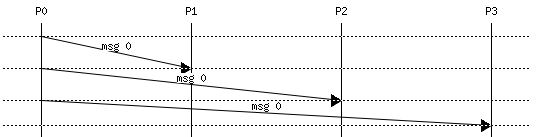
\includegraphics[scale=0.9]{basic.PNG}
	\caption{Diagram for the basic policy. The dashed horizontal lines represent the different rounds.}
	\label{fig:diagramBasic}
\end{figure}


\begin{itemize}
	\item The latency in this case, when there is no contention, will be $N-1$ (where is the number of processes in the system);
	\item For the case of $1$ sender, the throughput will be $\frac{1}{N-1}$.
\end{itemize}

\subsection{Tree}
	In this algorithm, each process that receives a message helps the original sender to spread it to the other processes. In order to simplify the implementation the simulator generates, for each message that will be broadcasted, a list containing pairs of $\left<sender, destination\right>$. For example, supposing the process $1$ wants to broadcast a new message, the simulator will generate a list $[\left<1, 2\right>, \left<1, 3\right>, \left<2, 4\right>]$ (process $1$ sends the message to processes $2$ and $3$, and process $2$ sends the message to process $4$). Although this may be unrealistic, we could implement this algorithm in real life by extending each message with a $level$ field (representing the current depth in the tree). This field is initialized with $0$ and, each time a process resends a message it increments this field. The next destination to which a process needs to send a received message is given by:
	
\begin{algorithm}
\begin{algorithmic}
\Function{NextDestination}{process, message, numProcesses}
	\State nextDest = ($process + 2^{message_{level}}$) \% numProcesses;
	\If{($nextDest \geq message_{sender}$) and ($nextDest \leq process$)}
		\State nextDest = $\emptyset$;
	\EndIf
	\State \Return nextDest;
\EndFunction
\end{algorithmic}
\caption{Tree Broadcast Policy}
\end{algorithm}

\begin{figure}[H]
	\centering
	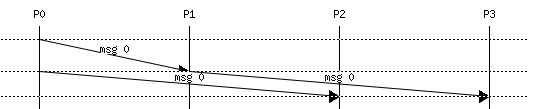
\includegraphics[scale=0.9]{tree.PNG}
	\caption{Diagram for the tree policy. The dashed horizontal lines represent the different rounds.}
	\label{fig:diagramTree}
\end{figure}

\begin{itemize}
	\item Since we double, at each round, the amount of processes that are able to spread the message, the latency (with no contention) will be $\log_2(N)$;
	\item For $1$ sender, the throughput will be $\frac{1}{log_2(N)}$.
\end{itemize}

\subsection{Pipeline}
	In this algorithm each process sends a message just once and then let the receiving process continue the broadcast, until all processes have received the broadcast. Although this does not have a latency as good as the \texttt{Tree} policy, the motivation is to distribute the work load among all processes, and let the first process free to send another message as soon as possible.
	
\begin{figure}[H]
	\centering
	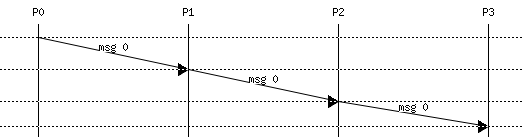
\includegraphics[scale=0.9]{pipeline.PNG}
	\caption{Diagram for the pipeline policy. The dashed horizontal lines represent the different rounds.}
	\label{fig:diagramPipeline}
\end{figure}
	
\begin{itemize}
	\item Since each process has to resend a message until the broadcast is done, the latency is $N-1$;
	\item For $1$ sender, as soon as the pipeline is full (the first message has been broadcasted), the throughput  will be $1$.
\end{itemize}

\newpage
\section{Total Order Broadcast}
\subsection{Properties}
	The desired protocol has the following properties (under the assumptions listed before):

\begin{description}
	\item[Validity] If a correct process p broadcasts a message m, then p eventually delivers m;
	\item[No duplication] No message is delivered more than once;
	\item[No creation] If a process delivers message m with sender s, then m was previously broadcasted by sender s;
	\item[Agreement] If a message m is delivered by some correct process, then m is eventually delivered by every correct process;
	\item[Total Order] If some process delivers message m2 after message m1, then every process delivers m2 only after it has delivered m1.
\end{description}

	The first four properties were already ensured by the base protocol, so the challenge is to extend it to provide the total order property.

\subsection{Protocol}
	To implement a total order, each process is extended with a logical clock (one per process), which is incremented each time a message is sent or received. Whenever a process $P_i$ wishes to send a message $m$, it uses its logical clock $C_i$ as a timestamp $m_{ts}$ for the message. Each process $P_k$ receiving this message synchronizes its own logical clock $C_k$ with the timestamp received ($C_k = \max(C_k, m_{ts}) + 1$), puts the received message in a waiting queue (a priority queue ordered by the timestamp and the sender id) and broadcasts an acknowledgement message containing the id of the received message and its timestamp. Each process that receives an ack can either:

\begin{enumerate}
	\item Create a fake entry in the waiting queue if it hasn't yet received a message with the corresponding id
	\item Update the timestamp of the corresponding entry in the waiting queue with the minimum between the current timestamp it has and the timestamp of the received ack
\end{enumerate}

	A process can deliver a message if and only if it has received all the acknowledgements for it and the message is the first in the waiting queue. These steps ensure that all processes will deliver all the messages in the same order, and is independent of the broadcast policy used (it can be combined with any of the three described in the previous session).
	
\subsection{Optimization Tradeoffs}
	Besides playing with the different broadcast policies, we found that there is small change we can make to \textbf{optimize the latency} of a broadcast (but \textbf{compromising the throughput}). In the described way, any process can start to send a message whenever they want. If we change this and let a process send a new message only when it has not message to deliver (the queue of messages waiting for acks is empty), there will be less acknowledgments being exchanged in the system (thus, less contention in the receive buffers). Another change that need to be done with this is that,the receiving process postpones the multicast of the ack, first trying to help broadcasting the message (if using the \texttt{Tree} or \texttt{Pipeline} policies).

\subsection{Evaluation}
	Using the results of the analysis made in section \ref{sec:policies} we could expect, in a first moment, that the best policies regarding latency and throughput would be the same when using a total order algorithm (i.e \texttt{Tree} with the best latency and \texttt{Pipeline} with the best throughput). However, after some tests we observed that, because of the acknowledgment messages, these results do not hold anymore.
	
	To verify that, we executed the total order simulator with the three policies (\texttt{Basic}, \texttt{Tree} and \texttt{Pipeline}) and three different configurations of events. The configurations are:
	
\begin{description}
	\item[singleMsg] the broadcast of just one message by one process
	\item[singleSender] one process broadcasts N messages in sequence
	\item[nSenders] all the process broadcast one message at the same time
\end{description}

Each pair of policy and configuration were executed for groups of size 4, 5, 10, 20 and 50, with the latency optimization previously  described actived and not (in the graphs, an $(O)$ after the policy name indicates it uses the original protocol version, and a $(L)$ indicates that it's using the latency optimization).

	The figures \ref{fig:avgLatPerPolicy} and \ref{fig:avgTpPerPolicy} show, respectively, the average latency and throughput obtained over the different cases tested. The figures \ref{fig:avgLatSingleMsg}, \ref{fig:avgLatSingleSender} and \ref{fig:avgLatNSenders} show the average latency obtained per test case while the figures \ref{fig:avgTpSingleMsg}, \ref{fig:avgTpSingleSender} and \ref{fig:avgTpNSenders} show the average throughput.
	
	From the figures \ref{fig:avgLatPerPolicy} and \ref{fig:avgTpPerPolicy}, we can see that the best protocols regarding the latency are indeed the latency-optimized ones (specially using the \texttt{Tree} policy). However, as expected, this optimization compromises the throughput. The best strategy for a good throughput is to keep the original implementation (sending a message whenever it's available) and use the \texttt{Tree} policy.
	
	It's also interesting to see that the \texttt{Pipeline} policy doesn't achieve, in general, a good performance in any of the cases. This can be explained because of the acknowledgment messages introduced for the total order algorithm: for each message a process receives it has two send one ack and resend the message itself, which has to be done in two different rounds. Summing this up with the contention generated by other processes' acks, its performance drastically drops.

\begin{figure}[htp]
  \centering
  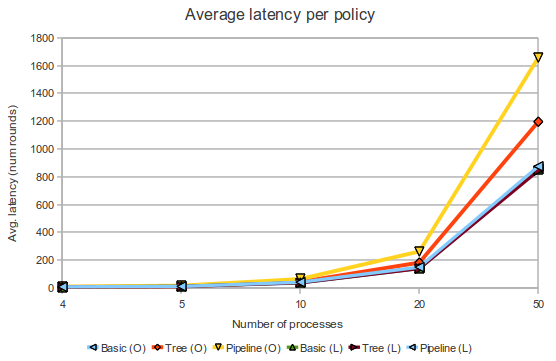
\includegraphics[scale=0.6]{avgLatPerPolicy.png}
	\caption{Average latency per policy (over all the test cases). The latency-optimized Tree policy has the lowest average latency.}
  \label{fig:avgLatPerPolicy}
\end{figure}

\begin{figure}[htp]
  \centering
  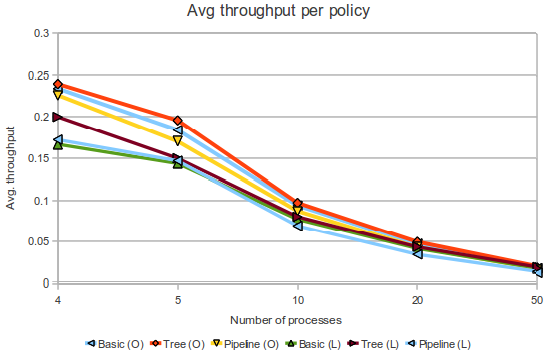
\includegraphics[scale=0.6]{avgTpPerPolicy.png}
	\caption{Average throughput (over all the test cases). The original-version Tree policy has the higher throughput.}
  \label{fig:avgTpPerPolicy}
\end{figure}


\begin{figure}[htp]
  \centering
  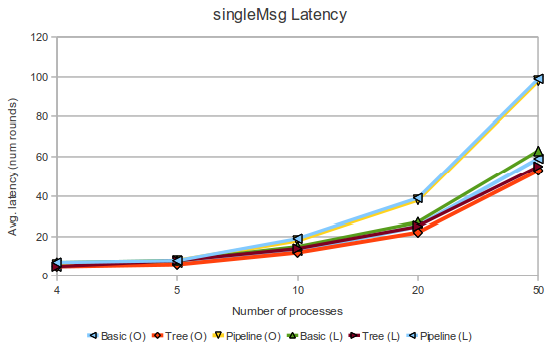
\includegraphics[scale=0.6]{avgLatSingleMsg.png}
	\caption{Average latency for the singleMsg case. Since just one message is sent, the latency-optimization does not have effect and and the two versions of each policy have similar performance. As expected after the theoretical analysis, the Tree policy has the lowest latency.}
  \label{fig:avgLatSingleMsg}
\end{figure}

\begin{figure}[htp]
  \centering
  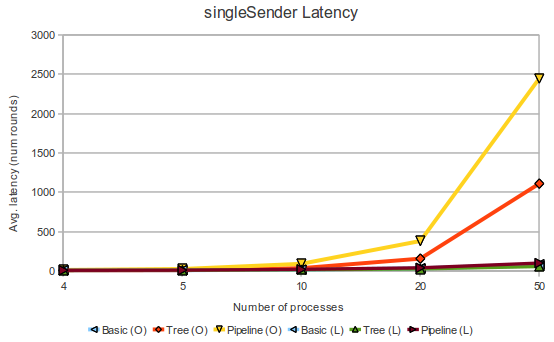
\includegraphics[scale=0.6]{avgLatSingleSender.png}
	\caption{Average latency for the singleSender case. In this case, the latency-optimization shows its effects. The latency-optimized versions obtain a much better performance than the original ones.}
  \label{fig:avgLatSingleSender}
\end{figure}

\begin{figure}[htp]
  \centering
  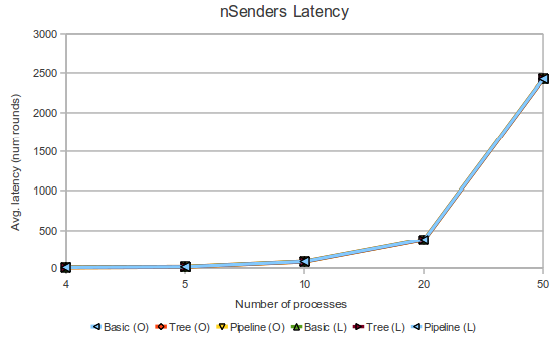
\includegraphics[scale=0.6]{avgLatNSenders.png}
	\caption{Average latency for the nSenders case. In this case all the processes start sending a message at the same time, so there's no room for the latency-optimization and all the policies have similar results.}
  \label{fig:avgLatNSenders}
\end{figure}

\begin{figure}[htp]
  \centering
  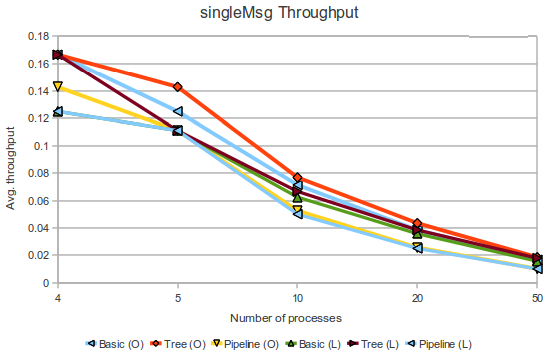
\includegraphics[scale=0.6]{avgTpSingleMsg.png}
	\caption{Average throughput for the singleMsg case. The best performance comes from the original-version Tree policy.}
  \label{fig:avgTpSingleMsg}
\end{figure}

\begin{figure}[htp]
  \centering
  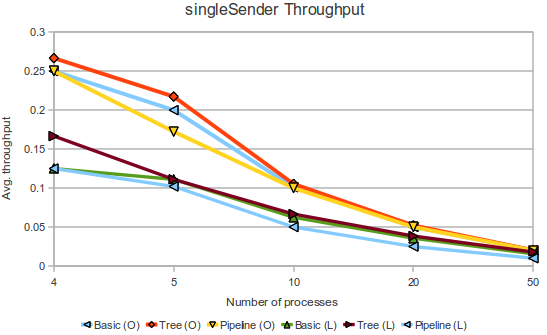
\includegraphics[scale=0.6]{avgTpSingleSender.png}
	\caption{Average throughput for the singleSender case. As expected the performance for the latency-optimized versions drastically drops and the original versions have best results.}
  \label{fig:avgTpSingleSender}
\end{figure}

\begin{figure}[htp]
  \centering
  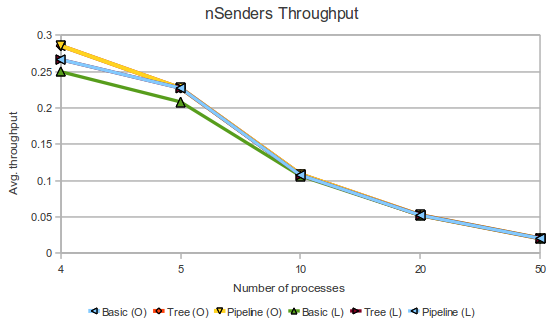
\includegraphics[scale=0.6]{avgTpNSenders.png}
	\caption{Average throughput for the nSenders case. Since the latency optimization be really used (because all the processes start sending at the same time), the results are close one to the other.}
  \label{fig:avgTpNSenders}
\end{figure}

\newpage
\section{Conclusion}
	In this project we designed and implemented a single-threaded, round-based simulator of broadcast protocols. This simulator runs according to the wanted specifications and can be executed with broadcast policies (\texttt{Basic}, \texttt{Tree} or \texttt{Pipeline}) with or without total order. 
	
	After running a few different tests to evaluate the broadcast algorithms, we can see that, while in the first version of the simulator (without total order) the \texttt{Tree} policy presented the lowest latency and the \texttt{Pipeline} policy, the highest throughput, the simple fact of introducing acknowledgement messages has changed this result. In our latency-optimized version (processes try, whenever is possible, to finish one broadcast before starting another) the lowest latency stayed with the \texttt{Tree} policy, but without this optimization the \texttt{Basic} policy showed the best results (the process that broadcast does not have to send acks to other processes). Regarding throughput, the \texttt{Tree} policy showed the higher rates in both the latency-optimized and the original version (but the higher throughput was observed in the version without blocking the sends).
	
	Even though the protocols developed have not so restrictive assumptions (the network is perfect and there are no crashes), this simulator offers a tool to understand and analyse the behaviour of different protocols for communicating distributed systems. However there are still many challenges to consider. Further work could be developed to take into account real life problems like network failures and crashes, thus introducing fault tolerance. 
 
\end{document}